% chap2.tex (Definitions)

\chapter{Text Classification with Deep Neural Networks}\label{TXT-CLASS}

\section{Brief Overview of Deep Learning}
Deep convolutional neural networks have seen an enormous amount of success on a wide
array of application, from scene interpretation to self-driving vehicles and art generation.
Natural language processing tasks are no exception to the range of problems
deep learning can solve, from sentiment analysis to language modeling. One very useful function of deep neural networks
is their ability to learn high-level features at each consecutive layer CITE[LE ET AL 2012].

One type of neural networks that is particularly good at learning features from the data is the convolutional neural network (CNN)CITE[LECUN 1989].
This type of network has achieved enourmous amounts of success on a wide array of applications CITE[Gu et al 2017]. A CNN learns a set of weights, or kernels, that are normally much smaller than the input size.
The difference in size forces the weights to have \textbf{sparse interaction} (i.e. a subregion of the input) versus the dense interaction
between every input with every output in traditional neural networks (i.e. vector-matrix multiplication). This sparse interaction
allows for features to be detected locally within the input (e.g. edge detection).
\textbf{Parameter sharing} allows for distinct outputs to be computed using the same set of weights. This drastically reduces
the amount of unique weights and to significantly increase network depth (i.e. deep networks) without the need
to increase the amount of training data.
These two design principles make CNN's poweful and efficient feature extractors.

Another type of deep neural network that has seen much success is the recurrent neural network (RNN). RNN's are designed to model data that display temporal structure, such as text and speech. By \textit{unfolding}
time-steps as a computational graph, the network can learn to model data along the time dimension, using at each time step the
raw input plus the output of the last time step's layer [Siegelman and Sontag 1995]. Because of the usually very deep structure of
the recurrent network, computation of the gradient via back propagation can lead to the \textit{vanishing gradient} problem, where the gradient
starts to shrink and become very close to zero as we back-propagate the errors. CITE[Sepp Hochreiter; Jürgen Schmidhuber (1997)] proposed
the \textbf{Long Short-Term Memory (LSTM)} recurrent network, a type of recurrent that essentially solves this problem with recurrent networks.
A recent and simpler variation of the LSTM network is the Gated Recurrent Unit (GRU) [Cho et al 2014], which performs comparably well CITE[Chung et al 2014].



\section{Word Embeddings}
Another significant achievement of deep learning for natural language processing is the neural probabilistic language model. CITE[BENGIO 2003 A NEURAL PROBABILISTIC LANGUAGE MODEL]
proposed a neural network to model the probability of a word given its context
$P(w_t|w_{t-k},\dots,w_{t-1})$

In their work, they addressed the curse of dimensionality, manifested by the fact that a test word sequence $(w_{t-k},\dots,w_{t})$
is likely to be different from all training sequences, by learning distributed representations of words. Words are represented as
dense continuous vectors called \textbf{word embeddings}.
Using word embeddings to model the likelihood of word sequences allowed generalization because the language model
would give high probability to unseen word sequences if they were made up of words semantically similar to already seen words.
Because of the of the underlying algorithm used to learn these word embeddings, similar words tend to lie closer to each other on
embedding space. Thus, word embeddings are said to capture semantic relations and encode more information than just a word identifier e.g.
a bag-of-words or one-hot vector representation.

\begin{figure}[h]
\caption{Visualization of embeddings using the T-SNE algorithm. Words with similar or related meanings
tend to lie close to each other in embedding space.}
\centering
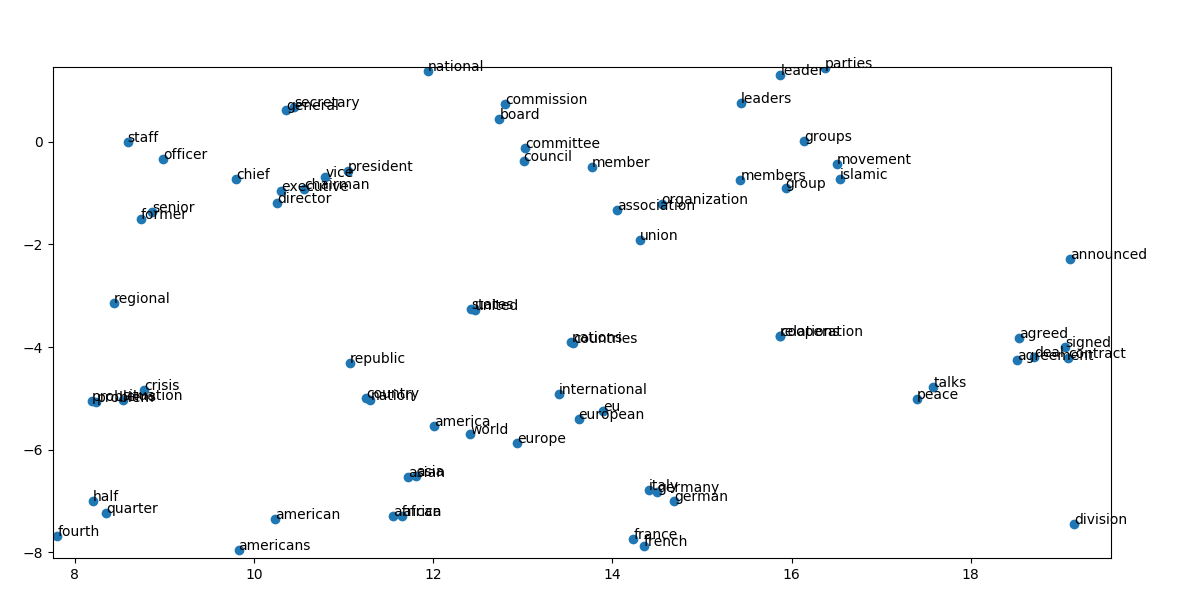
\includegraphics[width=0.5\textwidth]{EmbeddingViz.png}
\end{figure}

\section{Convolutional Neural Networks}
As described previously, convolutional neural networks are known for their abilities to learn high-level features from raw data. As input signals advance
forward through the network, they produce latent signals as linear conbinations with learned parameters, have non-linearities applied
to them, and have a pooling or selection mechanism based on simple functions such as the average or maximum operations [CITE ZHOU AND CHELLAPA 1988].

When dealing with image data, images are convolved with multiple filters, each convolution applied to overlapping subimages called as receptive fields.
This localized convolution process leads to discovery of low level features of images in the training set such as edges. As data
flows forward through the model, higher level features are discovered e.g. wheels or headlights in a vehicle image dataset.

These convolutional neural networks are comprised of \textit{feature maps}. A feature map is a \textbf{convolution} layer paired with a
\textbf{pooling} layer afterwards. The convolution stage creates \textit{activations}, whereas the pooling stage
reduces dimensionality and creates translation invariance.


\subsection{Input Representation: Word Embeddings for Convolutional Networks}
We can take advantage of word embeddings to apply convolutions to text in a fashion similar to convolutions with
image data and exploit the semantic information in the embeddings CITE[YUN 2014]. We apply the convolutions to overlapping sub-regions of the input text i.e. bi-grams, tri-grams, etc.
After convolution, we apply a non-linear function such as $max(0,x)$ and reduce data dimensionality
by pooling such as $x_{pool} = max(x_1,\dots,x_n)$.
Given a set of documents $\bm{s_1},...,\bm{s_m}$, we build a vocabulary $\mathbb{V}$ and a bag-of-words model from $\mathbb{V}$ to create a mapping $BoW:\mathbb{V} \mapsto \{1,...,|\mathbb{V}|\}$.
We represent a training document $\bm{s}$ as a sequence of integers $BoW(\bm{s})=$ $\bm{x} = x_1,...,x_k$, each integer being simply a word index
in $\mathbb{V}$. When the convolutional network receives this input sequence, each word index will be mapped to a corresponding embedding vector.

\begin{figure}[H]
\caption{Visualization of a feature map with a single kernel. In this example, the kernel convolves tri-grams, or windows of three words.
After convolution with all possible trigram context windows, max pooling is applied to reduce dimensionality.
Here, the pool size is 3. This process is repeated for as many filters in the layer e.g. 100 and their outputs are
concatenated horizantally to yield a matrix of size \textit{num filters} $\times$ (\textit{input length - pool size + 1}).}
\centering
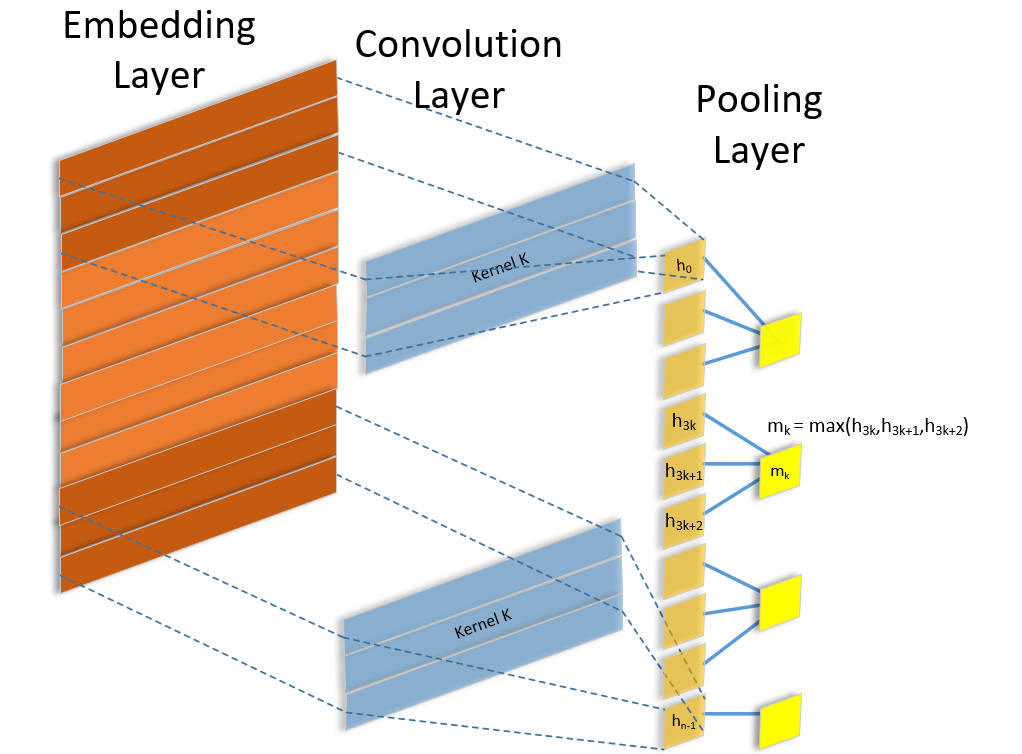
\includegraphics[width=0.5\textwidth]{FeatureMap.png}
\end{figure}
%%% Local Variables:
%%% mode: latex
%%% TeX-master: "thesis"
%%% End:
